\chapter{Structural Analysis}
\setlength{\parindent}{15pt}
\label{ch:stru_anal}

Connecting the various components of the UAV, the structure plays an essential role in the system design effort and therefore requires a careful analysis. Due to time constraints, the focus was put on the main wing internal structure, engine-wing connection and fuselage. The chapter presents the design approach that was used for both components independently, followed by the main assumptions and the analysis section. The latter is divided into the analysis of manoeuvre and gust loads, wing, fuselage and other parts such as tail and landing gear. Finally, the verification and validation procedures and an overview of the entire structure are presented.  

% =======================================================================================
\section{Design Approach}
\label{sec:desi_stru}

\begin{figure}[H]
    \centering
    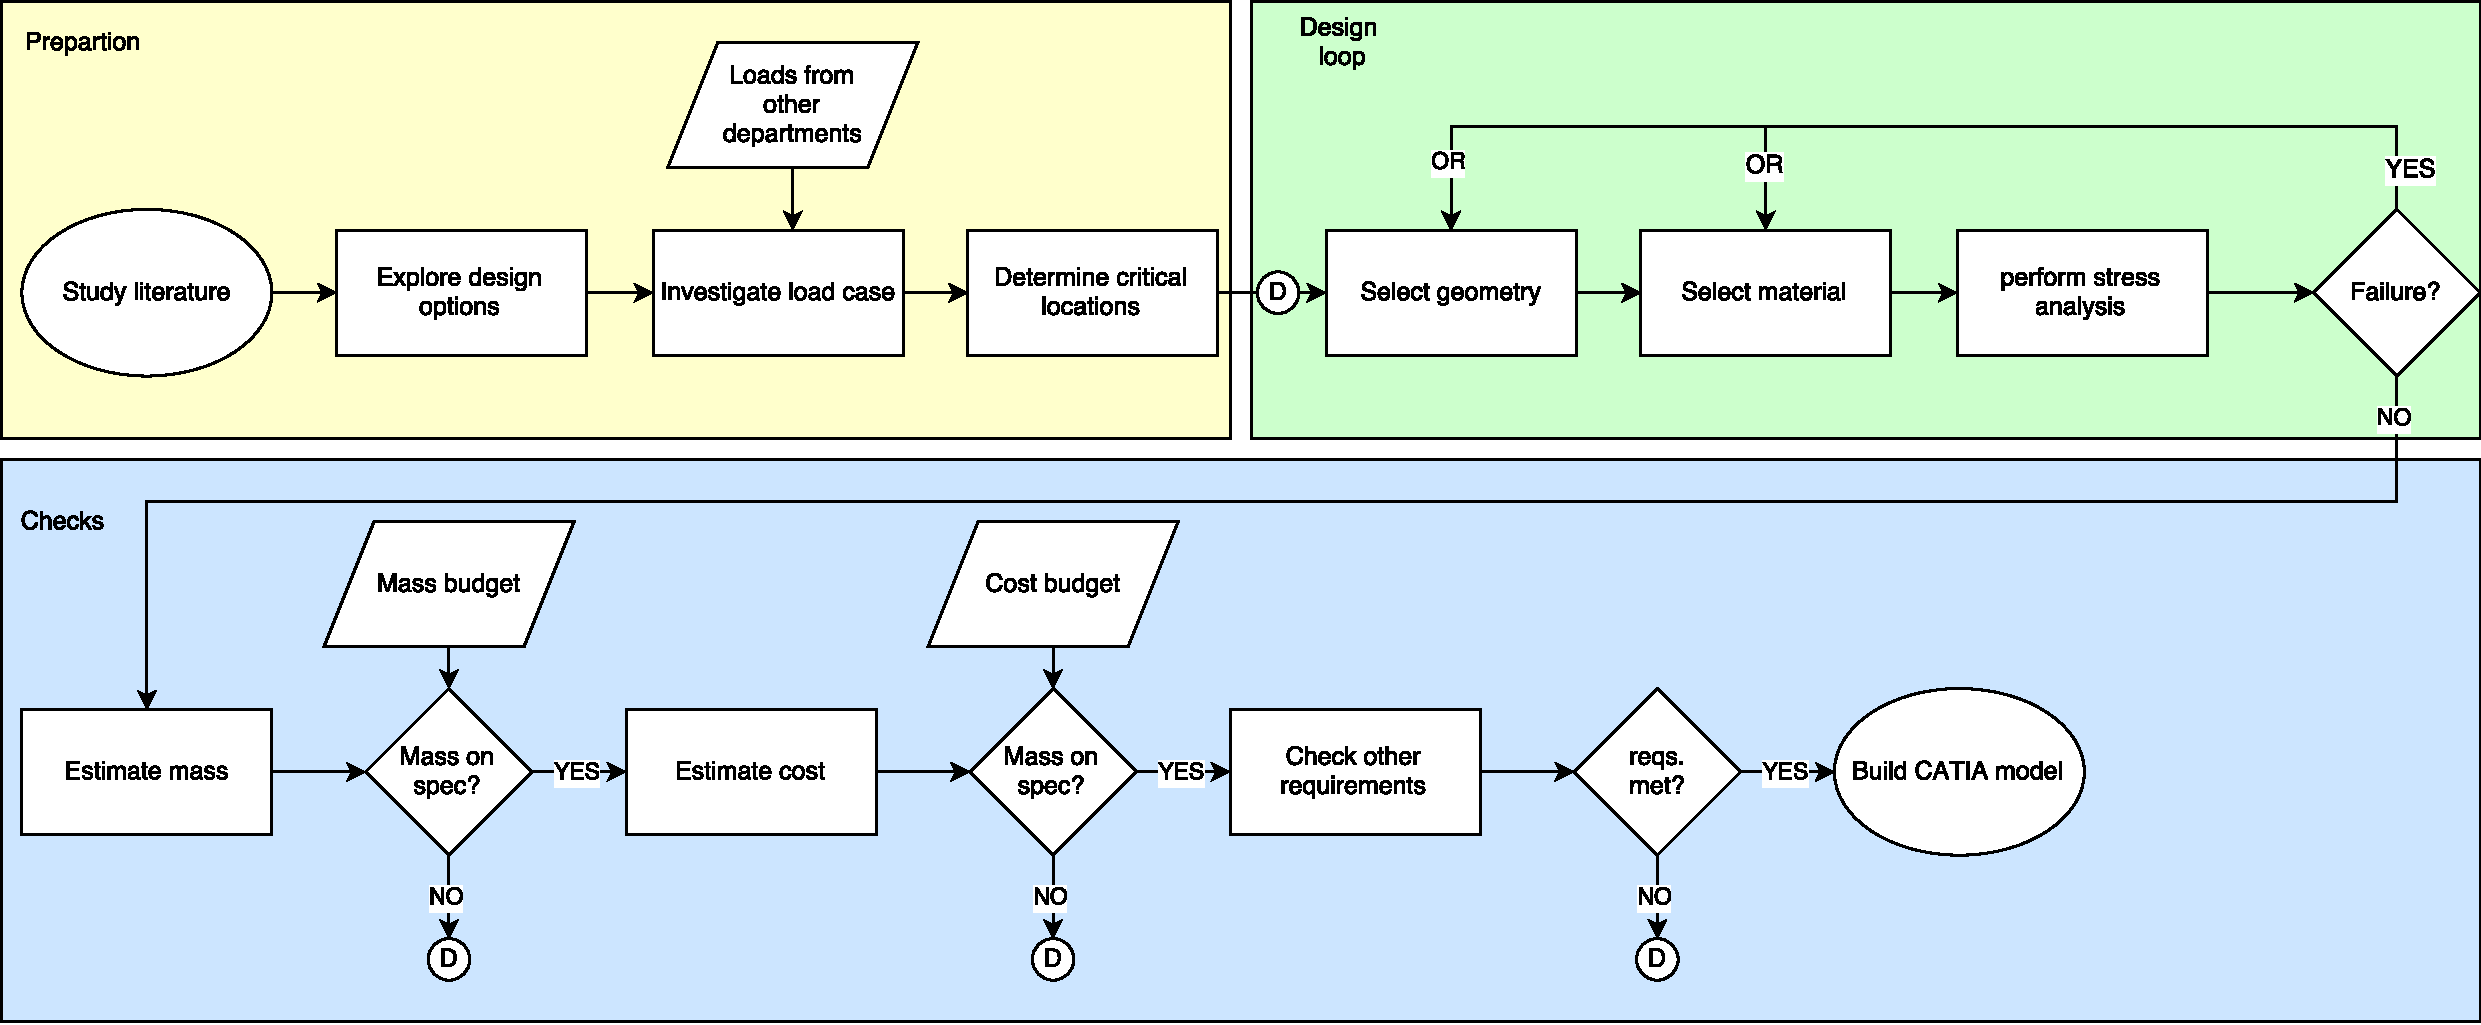
\includegraphics[width=1\textwidth]{Structures/Figures/struct_WFD}
    \caption{Work Flow Diagram}
    \label{fig:stru_WFD}
\end{figure}

The design approach that was chosen for the structural analysis and design of the UAV is presented in \autoref{fig:stru_WFD}. It can be split up into three different phases: a preparation phase in which the literate study is carried out to get a grasp of possible design choices and the various loads that act on airframe structures. Gathering data such as component weights, engine thrust and aerodynamic loads from other expert departments, it is possible to determine different load cases and find the maximum values for all locations of interest. Keeping other requirements in mind, the next steps are selecting a geometry which can be expected to perform well under the given loads and a material, and then run a stress analysis. Looking at the most critical combination of stresses, the structure can be checked for failure and re-designed if necessary. This iteration loop can be executed by either selecting a different geometry, a different material or both at the same time. If the structure is able to carry all loads without failing, various checks are performed to ensure compliance with other requirements. The first one is to calculate the total mass and compare it to the allocated budget. In case that it is to heavy, another design iteration loop has to be entered, which is indicated by a D in the figure. Next, a cost estimate is done to determine if the selected combination of geometry and material is producible within the budgetary constraints. Once those steps are completed, all other requirements such as environmental ones are considered and finally a CATIA model is created for verification and visualization purposes.

% =======================================================================================
\section{Assumptions}
\label{sec:assu_stru}

\begin{itemize}
    \item Maximum gust and manoeuvre loads do not occur simultaneously
    \item There are no axial forces on the main wing
    \item Stringers are only loaded in bending and axial direction
    \item The fuselage frames are loaded purely in shear
    \item The fuselage skin carries only shear stresses
    \item The area moment of inertia of a stringer about its centroid is negligible compared to its Steiner term.
\end{itemize}

% =======================================================================================
\section{Analysis}
\label{sec:anal_stru}

The purpose of this section is to present the steps that were taken to design the major structural components of the wing. It therefore covers preparatory aspects such as the determination of load factors and distributions, as well as descriptions of the methodology and results. Furthermore, considerations on components that were not designed in detail are given. 

% ---------------------------------------------------------------------------------------
\subsection{Manoeuvre and Gust Loads}

The shape and dimension of any structure depends on the loads that it is designed to withstand. In case of aircraft, loads heavily depend on the accelerations generated by manoeuvres and wind gusts, so an analysis as suggested in \cite{raymer} was performed for both situations. \autoref{fig:vn_diagram} shows the outcome, where the gust loads are indicated by solid lines and the manoeuvre loads by dotted lines. As can be seen in the figure, the gust loads are driving the design with a value of about +8.7 and -6.7 at cruise speed. These high values are mainly to the low wing loading of 31 kg/sqm and dwarf the manoeuvre loads of +4.4 and -1.8 found for typical general aviation utility aircraft in \cite{raymer}. For this reason a factor of 8.7 is applied to all loads, on top of the general safety factor of 1.5. 

\begin{figure}[H]
    \centering
    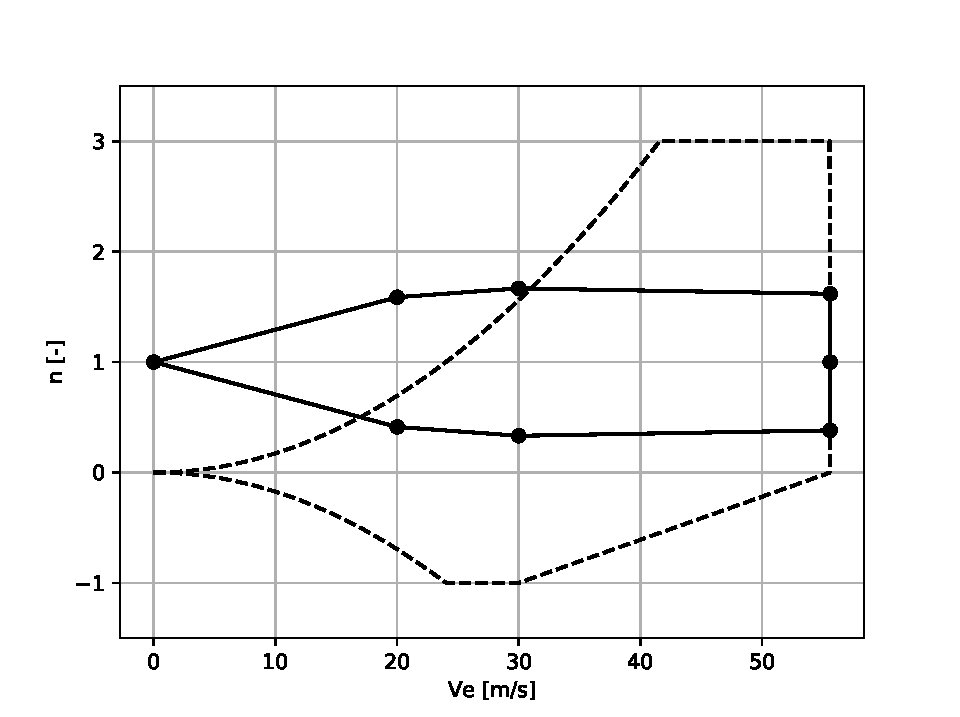
\includegraphics[width=0.7\textwidth]{Structures/Figures/vn_diagram}
    \caption{V-n Diagram}
    \label{fig:vn_diagram}
\end{figure}

% ---------------------------------------------------------------------------------------
\subsection{Main Wing}

The wing design involved almost all departments, the most prominent ones being aerodynamics for skin shape and aerodynamic loads, propulsion for thrust and control \& stability for engine and aileron positioning. This section deals with the load analysis, the chosen internal layout, a stress analysis including failure checks and some additional considerations which are not load-related.    

\paragraph{Load Analysis}

The loads acting on the main UAV wing can be separated into three groups: aerodynamic forces in horizontal flight, vectored engine thrust and weight contributions of various components. Not all of them act at the same time and in the same direction, so a separate analysis was performed for different flight conditions, and the most critical values identified for each part of the structure. The aerodynamic loads were imported directly from XFLR5, the wing weight approximated by distributing the allocated mass budget of the wing planform and the engine and fuselage connections modelled as point forces.   
\autoref{fig:FM_diags_z} shows the vertical shear force and corresponding bending moment diagram for half the wing span, starting from the axis of symmetry and ending at the wing tip. The dotted vertical lines indicate sections of interest, namely, from left to right: fuselage connection, engine pylon connection, wing disassembling point, inward aileron boundary, outward aileron boundary. The three curves represent the flight situations that were analysed: clean cruise conditions, manoeuvring with maximum aileron downward deflection and vertical climb at full engine thrust. In all cases the wing and engine weight produce a downward force and therefore a relieving bending moment, however, the lift and thrust forces are dominant. It was found that the largest maximum shear force and bending moment occurs while the UAV is manoeuvring, which is because the deflected aileron creates additional lift at a large distance from the root. On the contrary, the loads in VTOL phases are low due to the small moment arm. A similar analysis was performed in the horizontal plane, however, is not shown due to space constraints. % maybe appendix? 


\begin{figure}[H]
    \centering
    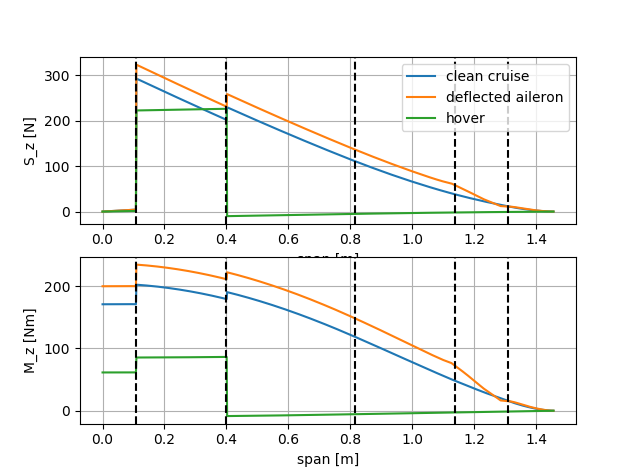
\includegraphics[width=1.0\textwidth]{Structures/Figures/FM_diags_z}
    \caption{Vertical Shear Force and Bending Moment Diagram}
    \label{fig:FM_diags_z}
\end{figure}

The torque around the y-axis exerted on the wing is displayed in \autoref{fig:FM_diags_T}. In this case the most critical condition is one engine being inoperative in VTOL mode, while the other one generates maximum thrust. The torques generated by the offset of the CP \nomenclature[A]{CP}{Center of Pressure} to the assumed shear centre of the load carrying structure is almost negligible.

\begin{figure}[H]
    \centering
    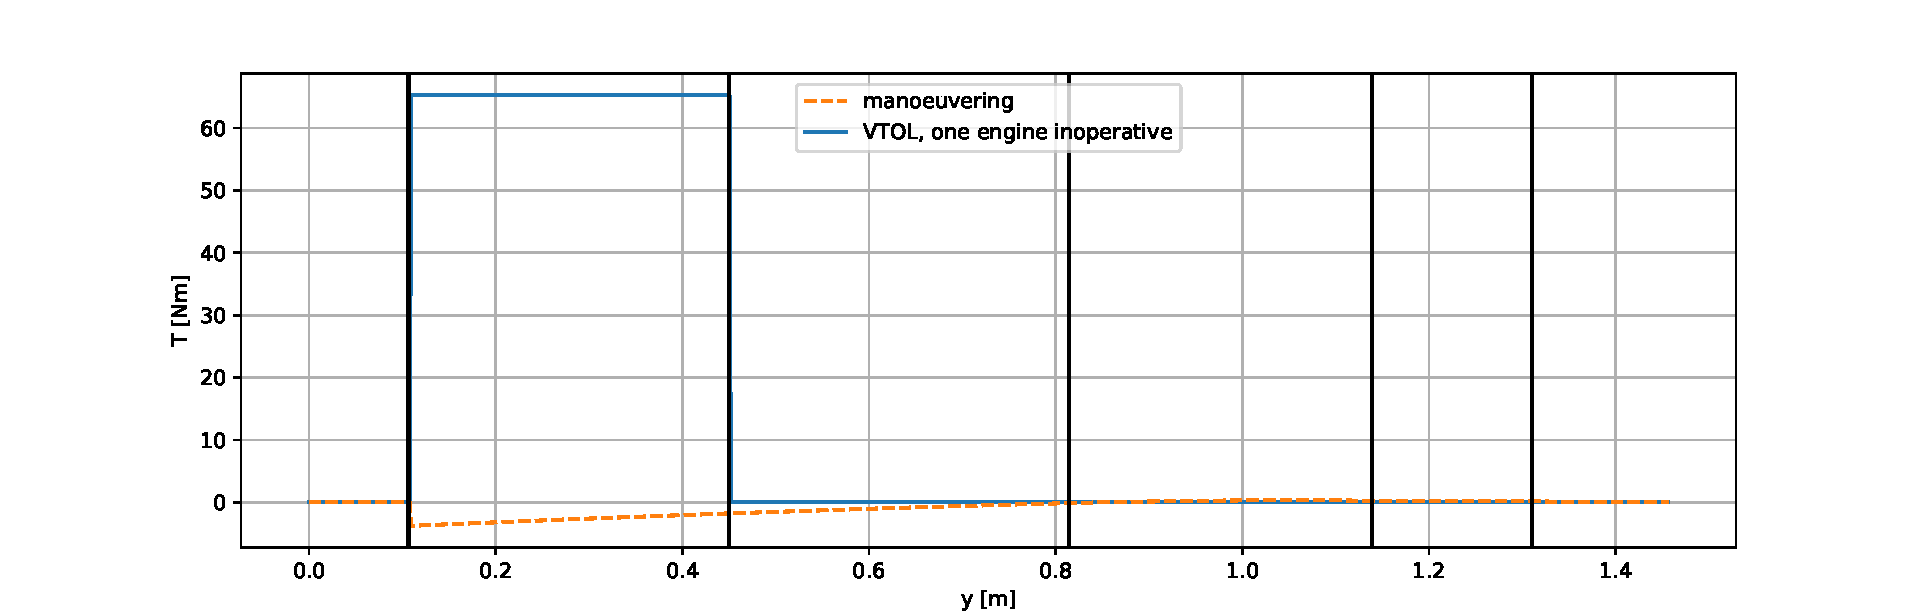
\includegraphics[width=1.0\textwidth]{Structures/Figures/FM_diags_T}
    \caption{Torque Diagram}
    \label{fig:FM_diags_T}
\end{figure}

\paragraph{Internal Layout}

After determining the loads that can be expect during operations, it is possible to design a structure that is able to carry them while also meeting the remaining subsystem requirements. After performing a literature study and consulting experts from the Atmos and 2seas UAV projects it was decided to design a load carrying tubular structure which is connected to a thick foam skin via a limited amount of ribs. The alternative would have been a classic wing box and stressed skin including stringers, but due to time constraints choosing a proven design seemed to be the better option. Furthermore, the chosen wing planform results in a low wing loading and having internal space for systems and fuel is not necessary, so the large volume and low strength of foam structures is not problematic. Since the only requirement on the skin is to not deform under aerodynamic loads, the main focus was put on sizing the tubular structures and choosing an appropriate material. \autoref{fig:wing_rendering} shows a rendering of the the main wing structure including the skin, the exact dimensions of the main parts can be found in \autoref{fig:w_internals}.

\begin{figure}[H]
\centering
\begin{minipage}{.5\textwidth}
    \centering
    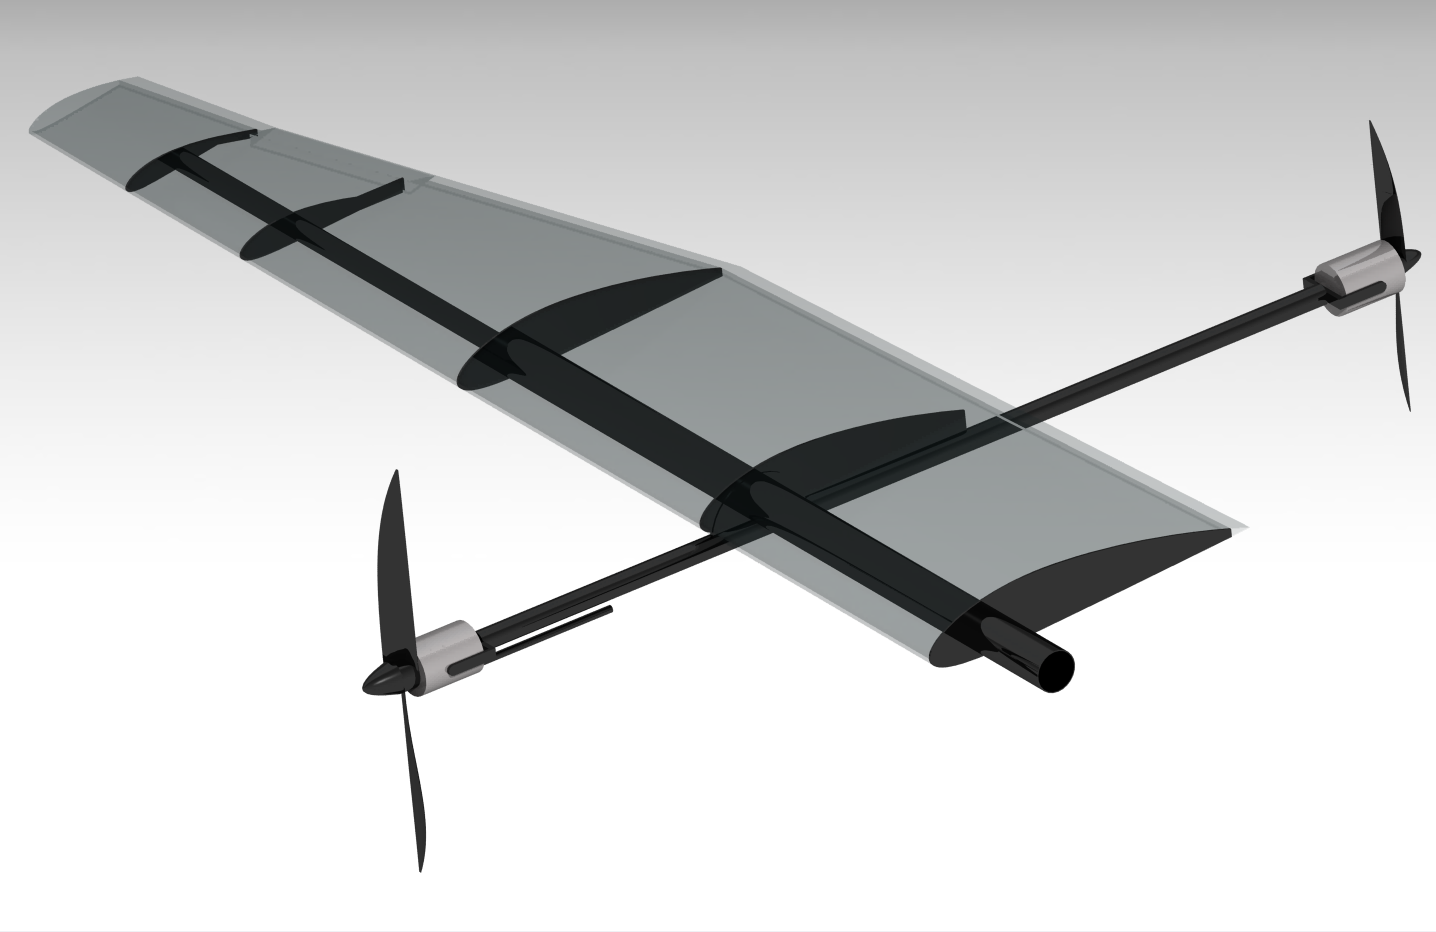
\includegraphics[width=\textwidth]{Structures/Figures/wing_rendering}
    \caption{Wing Structure}
    \label{fig:wing_rendering}
\end{minipage}%
\begin{minipage}{.5\textwidth}
    \centering
    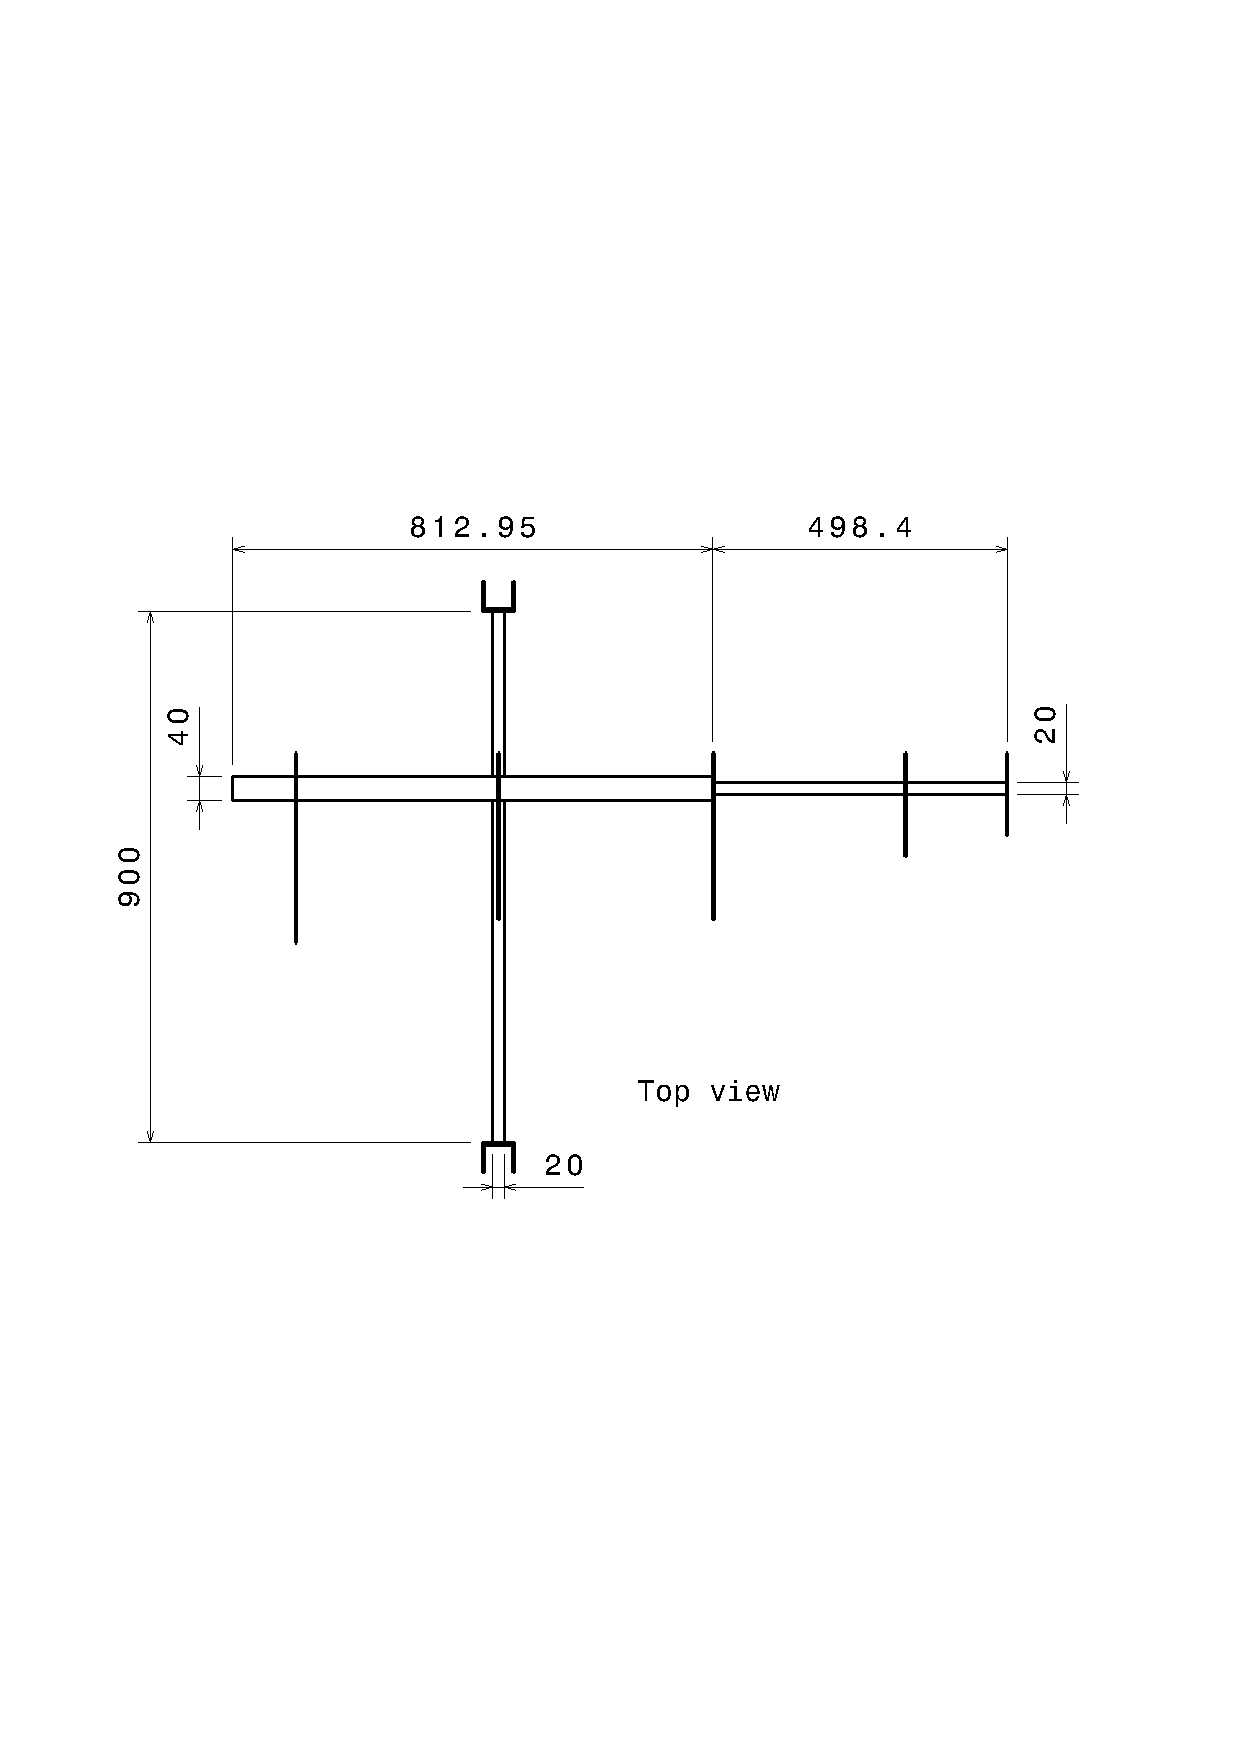
\includegraphics[width=\textwidth]{Structures/Figures/w_internals}
    \caption{Tube Dimensions}
    \label{fig:w_internals}
\end{minipage}
\end{figure}

The support structure can be broken up into three parts: the root tube, which is permanently connected to the fuselage, the detachable outer tube and the engine pylon. It was decided to use tubes with constant diameters because they feature a good torque resistance with minimal warping while being relatively simple to produce. The shear force and moment analysis showed that vertical loads outweigh horizontal loads, however, the weight benefit of having different MOIs per axis is not likely to justify the increase in complexity.
The connection between the root tube and engine pylon is achieved via a rib attached at this position. Spanning almost the entire chord at this wing section and fully enclosing the tube it is able to efficiently transfer all loads generated by upward and forward thrust of the engines and especially the torque in OEI \nomenclature[A]{OEI}{One Engine Inoperative} conditions. The connection between the root and outer tube has not been designed in detail yet, but is likely to have the smaller slide into the larger to transfer shear forces and moments and include some pins to prevent twisting. Also, the requirement for quick and easy disassembly would need to be taken into account. 
There are other ribs placed at the location where the wing intersects the fuselage skin, the location where the wing tip is detached, the outer edges of the aileron where the actuators are attached and at the end of the outer tube. Attached to the most outward rib is the wing tip, which fully consists of foam due to the low loads.

\paragraph{Material Selection}

Having determined the loads and selected an internal layout, the next step in the design process was to identify materials that do not fail under the applied stresses, while at the same time having low mass and cost. For the tubes in the wing the three materials presented in \autoref{tab:struct_materials} were considered because of their frequent application in the aerospace industry. Looking at the properties only, the uni-directional carbon-epoxy composite features superior performance in fibre direction and acceptable in the transverse, while having the lowest density of all three. For this reason it was decided to use this kind of composite, despite the very high cost per mass.     

\nomenclature[G]{$\sigma$}{Normal stress \nomunit{$N/m^2$}}
\nomenclature[G]{$\tau$}{Shear stress \nomunit{$N/m^2$}}

% Table generated by Excel2LaTeX from sheet 'Sheet1'
\begin{table}[htbp]
  \centering
  \caption{Structural Materials \cite{callister}}
    \begin{tabular}{llrrrrrrr}
    \toprule
    \bfseries Material  &\bfseries Type  &\bfseries Density &\bfseries E     &\bfseries G     &\bfseries $\sigma_{yield}$ &\bfseries $\sigma_u$ &\bfseries $\tau_u$ &\bfseries cost \\
          &       & [g/$cm^3$] & [Gpa] & [Mpa] & [Mpa] & [Mpa] & [Mpa] & [EUR/kg] \\
    \midrule
    Aluminium & Al 7075 & 2.8   & 71    & 27    & 103   & 570   & 330   & 11.6 \\
    Carbon-epoxy & T300/N5208  & 1.6   & 181   & 7.17  & N/A   & 1500  & 68    & 220 \\
    Glass-epoxy & E-glass & 1.8   & 38.6  & 4.14  & N/A   & 1062  & 72    & 33 \\
    \bottomrule
    \end{tabular}%
  \label{tab:struct_materials}%
\end{table}%

\autoref{tab:struct_foam} shows the engineering foams considered for the wing skin, Depron and expanded polypropylene (EPP). Both are common choices in the construction of scale models, and are therefore considered suitable to carry the aerodynamic loads.

% Table generated by Excel2LaTeX from sheet 'Sheet1'
\begin{table}[htbp]
  \centering
  \caption{Engineering Foams}
    \begin{tabular}{lrrr}
    \toprule
          &\bfseries Density &\bfseries E     &\bfseries cost \\
          &\bfseries [g/$cm^3$] &\bfseries [Gpa] &\bfseries [EUR/kg] \\
    \midrule
    Depron & 0.04  & 0.0144 & 34 \\
    EPP   & 0.1   & 0.013 & 17 \\
    \bottomrule
    \end{tabular}%
  \label{tab:struct_foam}%
\end{table}%


\paragraph{Stress Analysis}

A stress and subsequent failure analysis is crucial in every structural design effort. Having determined all loads and selected a preliminary geometry it is possible to calculate stresses, check for failure and iterate if necessary. \autoref{eq:sig_bend} shows the formulas which were used to determine the direct stresses on each point in the tubular cross-section due to moments in the vertical and horizontal plane:

\begin{equation}
\label{eq:sig_bend}
    {\sigma _{bend,x}} = \frac{{M \cdot x}}{I}
    \qquad
    {\sigma _{bend,z}} = \frac{{M \cdot z}}{I}
\end{equation}

\autoref{eq:tau} shows the shear stresses due to the applied torque and the shear forces in x- and z-direction, where $\theta$ is defined to run counter-clockwise from the negative x-axis:

\begin{equation}
\label{eq:tau}
    {\tau _{torque}} = \frac{T}{{2At}}
    \qquad
    {\tau _{shear,z}} = \frac{{{S_z}}}{{{I}}}t{r^2}\left[ {\cos \theta  - \cos \frac{\pi }{2}} \right]
    \qquad
    {\tau _{shear,x}} = \frac{{{S_x}}}{{{I}}}t{r^2}\left[ {\sin \theta } \right]
\end{equation}

\autoref{fig:root_sig} and \autoref{fig:root_tau} show the outcome of the stress analysis for the root tube-fuselage connection point, where the direct and shear stress components are superimposed separately. The maximum tensile stress is obtained at the bottom of the tube, slightly to the back. This is what can be expected due to the large aerodynamic load in combination with the forward engine thrust. Looking at the shear stress, the maxima are located at the front and the back of the tube, again due to the dominant lift forces. An analysis has been performed on the outer tube and engine pylon, resulting in very similar stress distributions.

\begin{figure}[H]
\centering
\begin{minipage}{.5\textwidth}
    \centering
    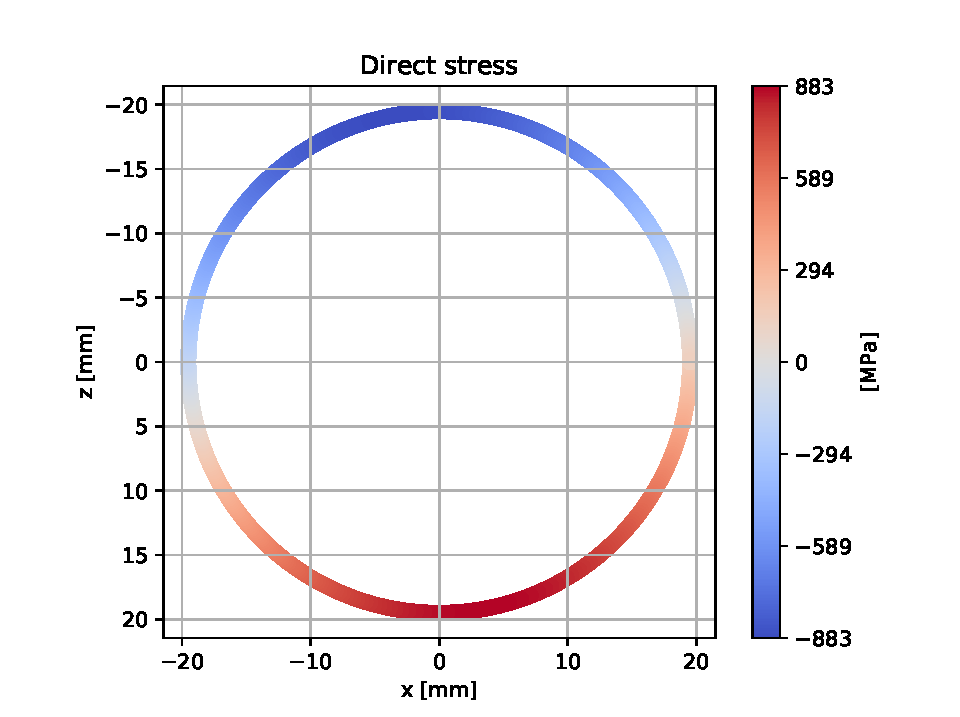
\includegraphics[scale=0.5]{Structures/Figures/root_sig}
    \caption{Root Direct Stresses}
    \label{fig:root_sig}
\end{minipage}%
\begin{minipage}{.5\textwidth}
    \centering
    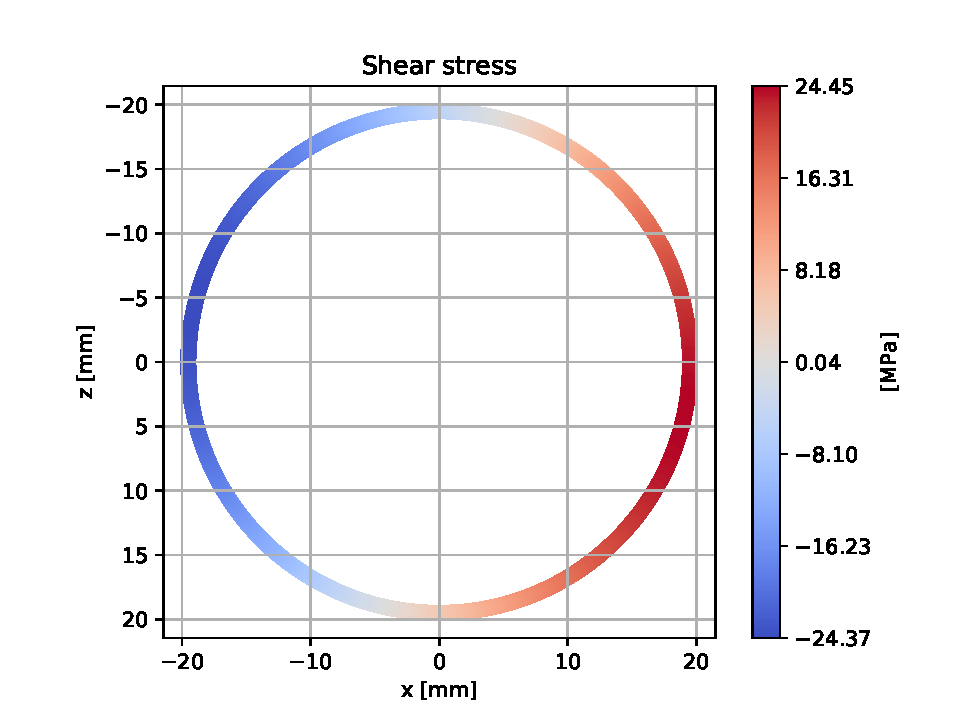
\includegraphics[scale=0.5]{Structures/Figures/root_tau}
    \caption{Root Shear Stresses}
    \label{fig:root_tau}
\end{minipage}
\end{figure}

\paragraph{Failure Analysis}

Similar to using the von Mises yield criterion to check if a ductile material fails, failure of composites can be checked by using the Tsai-Hill criterion \cite{pure_evil} presented in \autoref{eq:tsai_hill}. Substituting the longitudinal, transverse and shear stresses at each point in the cross-section and the material's maximum allowable values results in a distribution such as \autoref{fig:root_failure}. As can be seen, all values are well below 1.0, so the structure is not likely to fail in the modes considered.  

\begin{equation}
\label{eq:tsai_hill}
    {\left( {\frac{{{\sigma _L}}}{{{\sigma _{Lu}}}}} \right)^2} + {\left( {\frac{{{\sigma _T}}}{{{\sigma _{Tu}}}}} \right)^2} - \frac{{{\sigma _L}}}{{{\sigma _{Lu}}}} \cdot \frac{{{\sigma _T}}}{{{\sigma _{Lu}}}} + {\left( {\frac{{{\tau _{LT}}}}{{{\tau _{LTu}}}}} \right)^2} \leqslant 1
\end{equation}

\begin{figure}[H]
    \centering
    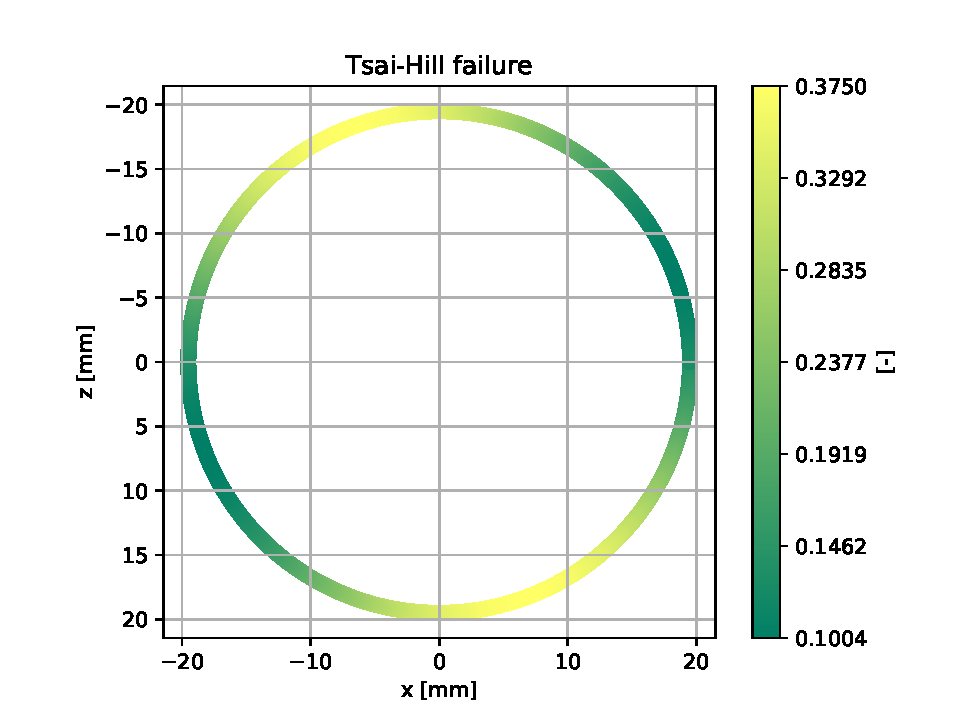
\includegraphics[width=0.5\textwidth]{Structures/Figures/root_failure}
    \caption{Root Tube Failure Check}
    \label{fig:root_failure}
\end{figure}

\autoref{tab:tube_failure} shows the outcome of the stress and failure analysis for all three tubes. The outer tube has a direct stress close to the ultimate, resulting in a maximum Tsai-Hill failure value of 0.732. The engine pylon appears to be over-designed since the stresses are far below the maximum allowable, however, in a pusher-prop configuration it needs to handle the compressive stresses generated by the engine and provide internal space for electric wires.  

% Table generated by Excel2LaTeX from sheet 'Sheet2'
\begin{table}[htbp]
  \centering
  \caption{Stress and Failure Overview}
    \begin{tabular}{lrrrrr}
    \toprule
          &\bfseries diameter &\bfseries thickness &\bfseries $\sigma_{max}$ &\bfseries $\tau_{max}$ &\bfseries Tsai-Hill \\
          &\bfseries [mm]  &\bfseries [mm]  &\bfseries [MPa] &\bfseries [MPa] &\bfseries [-] \\
    \midrule
    Root tube & 40    & 1     & 883   & 24.5  & 0.375 \\
    Outer tube & 20    & 2     & 1283  & 10.6  & 0.732 \\
    Engine Pylon & 20    & 1     & 267.8 & 4.3   & 0.031 \\
    \bottomrule
    \end{tabular}%
  \label{tab:tube_failure}%
\end{table}%

%\paragraph{Other Considerations}
% wires in tubes
% smooth surface by polymer
% vibrations


% ---------------------------------------------------------------------------------------
\subsection{Fuselage}

\paragraph{Load Analysis}
In the load analysis of the fuselage, the forces and moments about the aircraft's principal axes are determined for a wide range of operational situations. Out of these, the most critical ones are selected to guide the design.

The foreseeable loads to which the fuselage will be subjected during the UAV's operational life are divisible into:

\begin{itemize}
    \item In-flight manoeuvre loads
    \item Gust loads
    \item Take-off and landing loads
    \item Ground handling loads
\end{itemize}

This analysis mainly focuses on the in-flight manoeuvre and gust loads. The maximum design load factors for both gust and manoeuvre loads are 8.7 and 3.0 respectively, see \autoref{fig:vn_diagram}. A safety factor of 1.5 is also included to ensure safe operations within the design limits and to have a safety margin. 

The strongest bending moment about the y-axis as well as the highest vertical shear force loading are encountered during a maximum load factor pull up from a dive whilst in the fixed wing flight mode. The corresponding internal shear force and bending moment throughout the fuselage are depicted in \autoref{fig:fsmd}. The vertical dashed lines indicate the positions of the start of the payload bay, the fuselage mounted battery pack, the wing-fuselage connection, the end of the payload bay and the tail-fuselage connection. The maximum vertical shear force is 1642.3 N  downwards just  fore of the wing-fuselage connection. The maximum bending moment is 606.0 Nm and also occurs at the wing-fuselage connection. The maximum torque on the fuselage is 60.9 Nm and at full thrust the highest axial tensional load is 246 N.

The strongest bending moment about the z-axis and horizontal shear load occur in the case of a one engine out scenario, in which the remaining engine is operating at full thrust. The internal bending moment $M_{z}$ and the shear force $S_{y}$ are 83 Nm and 81.6 N respectively in this case.







\begin{figure}[H]
    \centering
    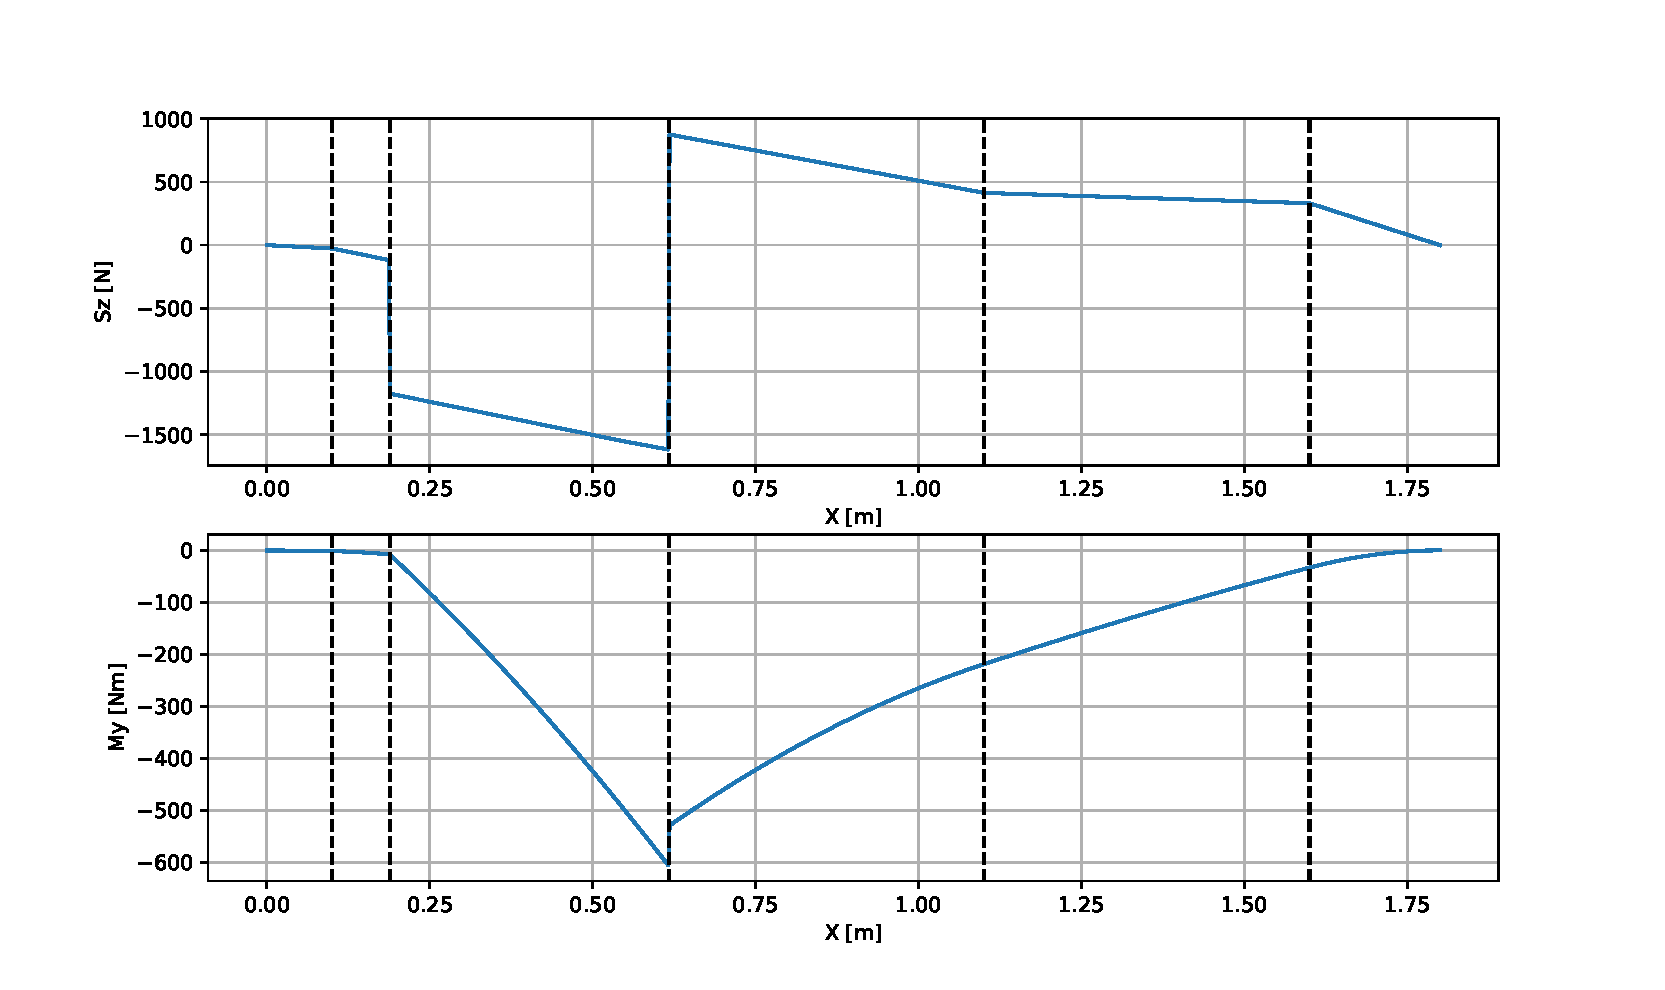
\includegraphics[width=1.1\textwidth]{Structures/Figures/fus_smd}
    \caption{Vertical Shear Force and Bending Moment in the Fuselage}
    \label{fig:fsmd}
\end{figure}



\paragraph{Internal Layout}
\autoref{fig:inter} shows the internal layout of the vehicle. On the bottom floor of the centre section of the fuselage the payload bay is located. It is accessible from the underside and has dimensions of 0.15 x 0.15 x 1.0 m (width x height x length). In the nose section two 0.082 x 0.045 x 0.162 m battery packs are situated in front of the main avionics. The wing intersects the fuselage above the payload bay so that the internal load carrying structural elements of the wing are not interrupted. Along the length of the fuselage seven frames are placed at the main locations of load introduction into the fuselage and to interrupt some large singular pieces of skin that would otherwise buckle under compression stresses. Frame one guides the inertial loads from the avionics and batteries into the rest of the structure. Frames two and six disperse the loads introduced by the front and rear landing skids. The loads generated by the main wing will be introduced into the fuselage via frames three and four, whilst frame seven will introduce the tail loads into the fuselage structure. Frame 5 protects the skin in the centre part of the fuselage around the payload from buckling. In the longitudinal direction, a total of seven stringers run between frames one to seven. Only one is visible in \autoref{fig:inter}. 

\begin{figure}[H]
    \centering
    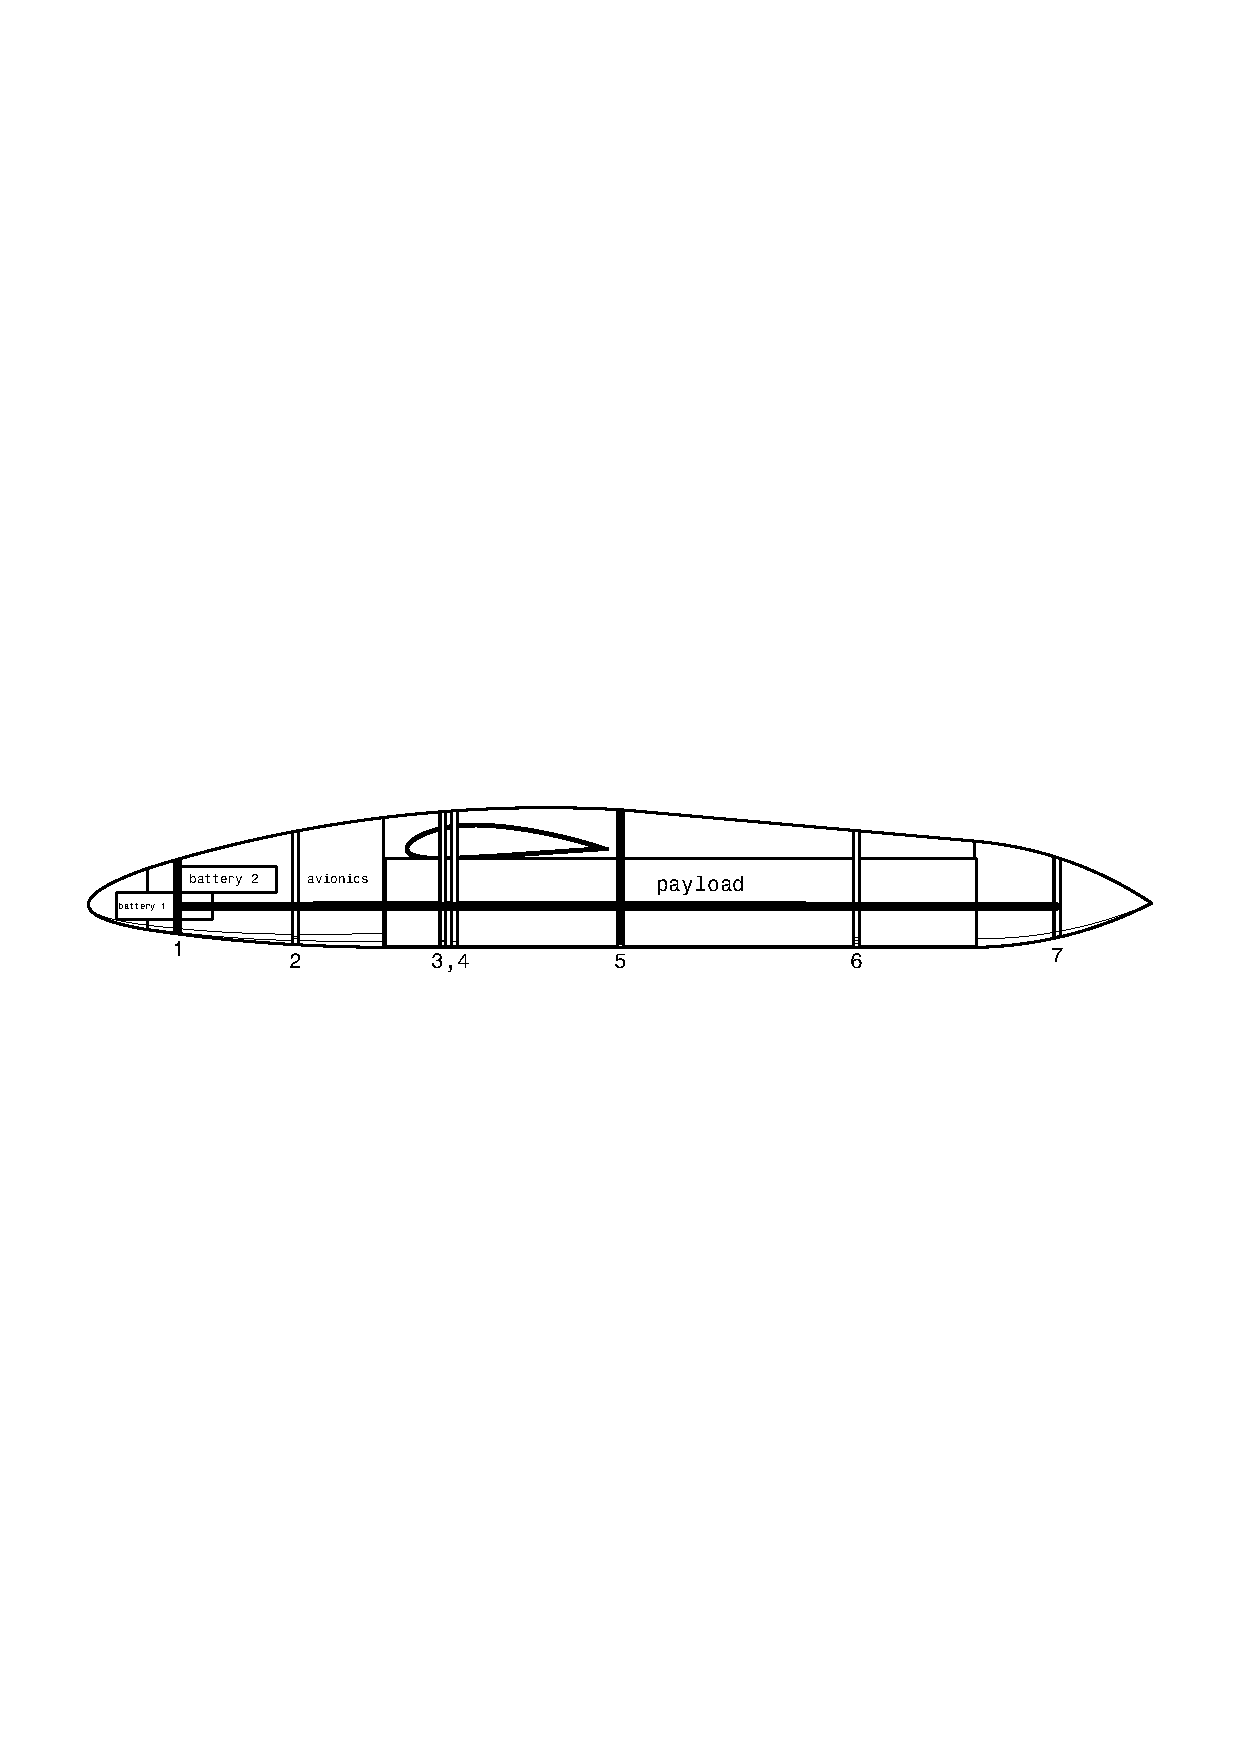
\includegraphics[width=0.75\textwidth]{Structures/Figures/Drawing2}
    \caption{Internal Layout of the Hybrid UAV}
    \label{fig:inter}
\end{figure}

\begin{figure}[H]
    \centering
    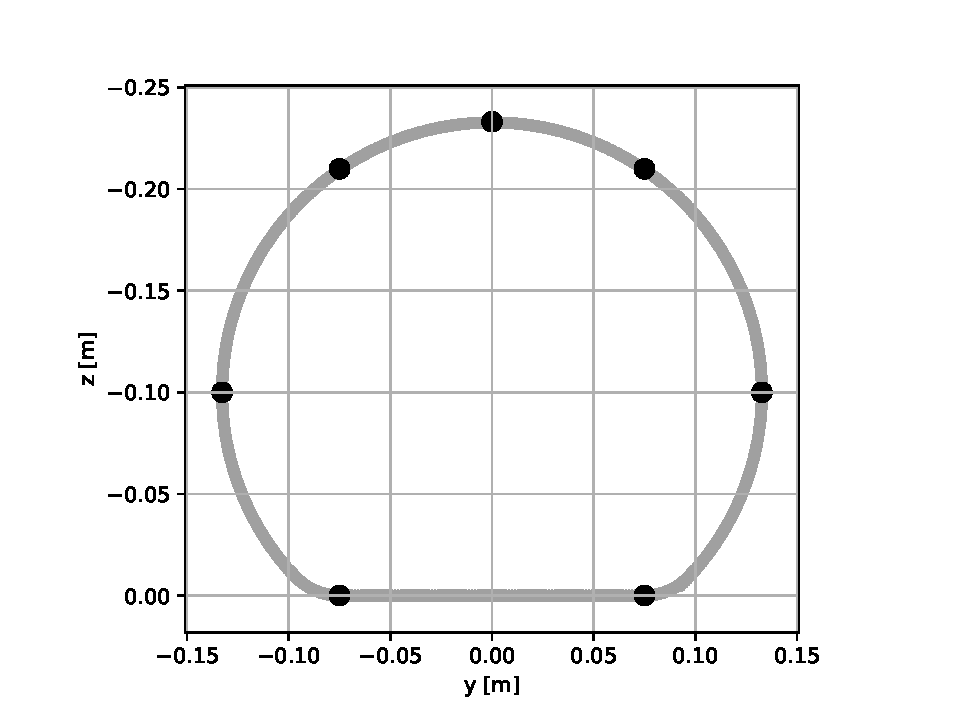
\includegraphics[width=0.75\textwidth]{Structures/Figures/figure_2}
    \caption{Stringer locations on frame 4}
    \label{fig:stringers}
\end{figure}

Between the first and seventh frame a total of seven stringers run in the longitudinal direction. Their positions are shown in \autoref{fig:stringers}

\paragraph{Stress and Failure Analysis}

The stresses resulting from the loads discussed before are analysed by applying the method of structural idealisation \cite{megson}. The bending moments on the fuselage which are in reality resisted by both the longitudinal stringers and the fuselage skin are assumed to be carried by a series of concentrations of area known as booms. These have a cross-sectional area that accounts for both the stringers and the skin in between a boom and its neighbouring counterparts as can be seen from \autoref{eq:boom}.

\begin{equation}
\label{eq:boom}
    B_{1} = B_{stringer}+\frac{t_{D}b}{6}\left ( 2+\frac{\sigma _{2}}{\sigma _{1}} \right )
\end{equation}
\nomenclature[B]{$B$}{Boom area}
\nomenclature[G]{$\sigma_{x}$}{Normal stress in x-direction}
\nomenclature[B]{$t_{D}$}{Skin panel thickness}
\nomenclature[B]{$t$}{Skin thickness}
 The contribution of the skin to the boom areas is based on the change in stress between the booms as to constrain equal elastic deformation in both the original and the idealised structure. The second moments of area of the idealised structure about the neutral axes are evaluated by taking only the Steiner terms of the booms. Then, the bending stress in each boom can be determined with \autoref{eq:sig_bend}.
 
  \begin{equation}
     \label{eq:directstress}
     \sigma _{x} = \frac{T_{max}}{\sum_{r=1}^{7} B_{r}}
 \end{equation}

\nomenclature[B]{$T_{max}$}{Maximum thrust}

The highest total direct stress is acquired by adding the stresses caused by the strongest axial load, calculated with \autoref{eq:directstress}. An overview of the boom stresses at the wing-fuselage connection can be found in \autoref{tab:struct_direct}. The bottom section of the fuselage which lies beneath the neutral axes of bending is loaded in tension. On the other hand, the top part of the fuselage is loaded in compression. This means that in the lower section the tensional direct stresses from the axial loads increase the total stress. Conversely, in the upper section the direct loads actually provide a small amount of stress relief.





\begin{table}[htbp]
  \centering
  \caption{Fuselage Boom Stresses at x=0.617 m}
    \begin{tabular}{lrrr}
    \toprule
    \bfseries Boom      &\bfseries $\sigma_{x_{bending}}$ [MPa]&\bfseries $\sigma_{x_{axial}}$ [MPa]    &\bfseries $\sigma_{x}$ [MPa] \\
    \midrule
    $B_{1}$  &  21.6 &  0.7  & 22.3  \\
    $B_{2}$  & 1.6 &  0.7  & 2.3 \\
    $B_{3}$  & -16.1 & 0.7   & -15.4 \\
    $B_{4}$  &  -17.6 & 0.7   & -16.9 \\
    $B_{5}$  & -10.8 & 0.7   & -10.1 \\
    $B_{6}$  & 11.1 &   0.7 & 11.8 \\
    $B_{7}$  & 27.0&  0.7  &  27.7\\
    \bottomrule
    \end{tabular}%
  \label{tab:struct_direct}%
\end{table}%

 
The fuselage skin and frames are carrying the shear and torsional loads acting on the vehicle. They are analysed for shear stress at the wing fuselage intersection, where both the torque and shear loading are highest throughout the structure. In accordance with the structural idealisation method from \cite{megson}, the shear flow is assumed to be constant between booms. The shear flow in a piece of skin past boom $n$ is then given by \autoref{eq:shear_flow}
\begin{equation}
\label{eq:shear_flow}
q_{s_{n}} = - \frac{S_{y}}{I_{zz}}    \sum_{r=1}^{n} B_{r}y_{r} - \frac{S_{z}}{I_{yy}} \sum_{r=1}^{n} B_{r}z_{r} 
\end{equation}

\nomenclature[B]{$S_{y}$}{Shear force in y-direction}
\nomenclature[B]{$S_{x}$}{Shear force in x-direction}
\nomenclature[B]{$S_{z}$}{Shear force in z-direction}
\nomenclature[B]{$q_{s}$}{Shear flow}

The vertical shear force's line of action passes through the shear centre as it lies in the plane of symmetry. The horizontal shear loads do in reality induce additional shear stresses on the fuselage as both the engines and the vertical tail do not generate forces in line with the shear centre. Therefore the horizontal shear loads are treated as a superposition of cases of pure shear and torsion. The location of the shear centre is approximated by the centroid of a circle with a radius equivalent to that of the actual fuselage. Although this introduces a small error in the model, it is only minor since the horizontal shear forces are an order of magnitude smaller than their vertical counterparts. Next, the shear flow due to a torsional load is calculated with \autoref{eq:shear_torq}
\begin{equation}
\label{eq:shear_torq}
    T = 2Aq
\end{equation}

\nomenclature[B]{$T$}{Torque}
\nomenclature[B]{$A$}{Enclosed area}


Now, the actual shear stresses are found by dividing the shear flow in each section by the skin thickness, which is 0.5 mm (\autoref{eq:qtau}).

\begin{equation}
\label{eq:qtau}
    \tau = \frac{q}{t}
\end{equation}

The resulting stresses are shown below in \autoref{tab:struct_shear}. 
\begin{table}[htbp]
  \centering
  \caption{Fuselage Shear Stresses}
    \begin{tabular}{lrrrr}
    \toprule
    \bfseries Section      &\bfseries $\tau_{S_{z}}$ [MPa]&\bfseries $\tau_{S_{y}}$ [MPa]    &\bfseries $\tau_{M_{x}}$ [MPa] &\bfseries $\tau$ [MPa] \\
    \midrule
    $s_{1,2}$  &  -6.8 & $-1.1\cdot 10^{-1}$ & 1.1 & -5.7  \\
    $s_{2,3}$  & -7.8 & $2.4\cdot 10^{-1}$ &  1.1 & -6.9\\
    $s_{3,4}$  & -3.6 & $3.8\cdot 10^{-1}$ &  1.1 & -2.8\\
    $s_{4,5}$  &  3.6 & $3.8\cdot 10^{-1}$ & 1.1 &  4.4\\
    $s_{5,6}$  & 7.8 &  $2.4\cdot 10^{-1}$ &  1.1 & 8.7\\
    $s_{6,7}$  & 6.8 &  $-1.2\cdot 10^{-1}$ &  1.1 & 7.8\\
    $s_{7,1}$  & $-1.2\cdot 10^{-3}$& $-4.26\cdot 10^{-17}$  & 1.1 & 1.1\\
    \bottomrule
    \end{tabular}%
  \label{tab:struct_shear}%
\end{table}%
Since the skin and frames are assumed to only carry shear stresses, whilst the stringer resist all the axial and bending loads, they can be compared directly to the materials ultimate stress. As \autoref{tab:struct_materials} shows, Glass-epoxy is strong enough for to endure all of the stresses shown in \autoref{tab:struct_shear} and \autoref{tab:struct_direct}.

\paragraph{Material}

The stringers, fuselage frames and skin are to be made out of a glass fibre epoxy composite. This material was chosen over aluminium and carbon fibre composites because it combines low cost and high strength. As \autoref{fig:stru_WFD} shows, the material and geometry where first selected and then the stress analyses and budget checks were performed. Every combination of geometry and aluminium considered either failed or violated the mass budget. Since the extra strength that carbon fibre offers over glass fibre was not needed according to the stress analysis, Glass fibre was chosen because it is significantly less expensive.

% ---------------------------------------------------------------------------------------
\subsection{Tail}

Due to limited resources it was not possible to design the vertical and horizontal tailplanes with the same level of detail as the main wing and fuselage, however, a preliminary internal structure was established to determine the expected cost and mass. For the main wing the combination of carbon fibre tubes for load transfer and engineering foam for having an aerodynamic shape proved to be beneficial, so it was decided to use a similar concept for the tail. The vertical tailplane would therefore consist of a a hollow carbon fibre tube surrounded by a solid layer of foam. Attachment of the rudder hinge and actuator would ideally be directly at the tube, however, additional ribs could be placed if necessary. The tube supporting the horizontal tail is then fixed to the vertical one, with a similar hinge/actuator placement for the elevator.  


% ---------------------------------------------------------------------------------------
\subsection{Landing Gear}

Since the UAV is expected to take off and land vertically, the landing gear design can be very simple and light. Two aerodynamically shaped blocks of rubber are attached to the fuselage frames number 2 and 6 in \autoref{fig:inter} to dampen the impact loads that occur during landings. The ground clearance is very limited with this configuration, however, the sensor layout allows for scanning of downward surfaces and can therefore ensure that the ground is smooth enough for safe landings. Furthermore, the skin at the belly could be reinforced if frequent outdoor landings are required by a customer.   
Tipping over onto the wing tips is preventing by installing carbon fibre rods to the front front engines, as shown in \autoref{fig:ground_clearance}. This configuration ensures a side tip angle of no more than 5.75 degrees and, tilting backward with the engine casing, stores in a aerodynamically favourable position without the need of extra mechanisms.


\begin{figure}[H]
    \centering
    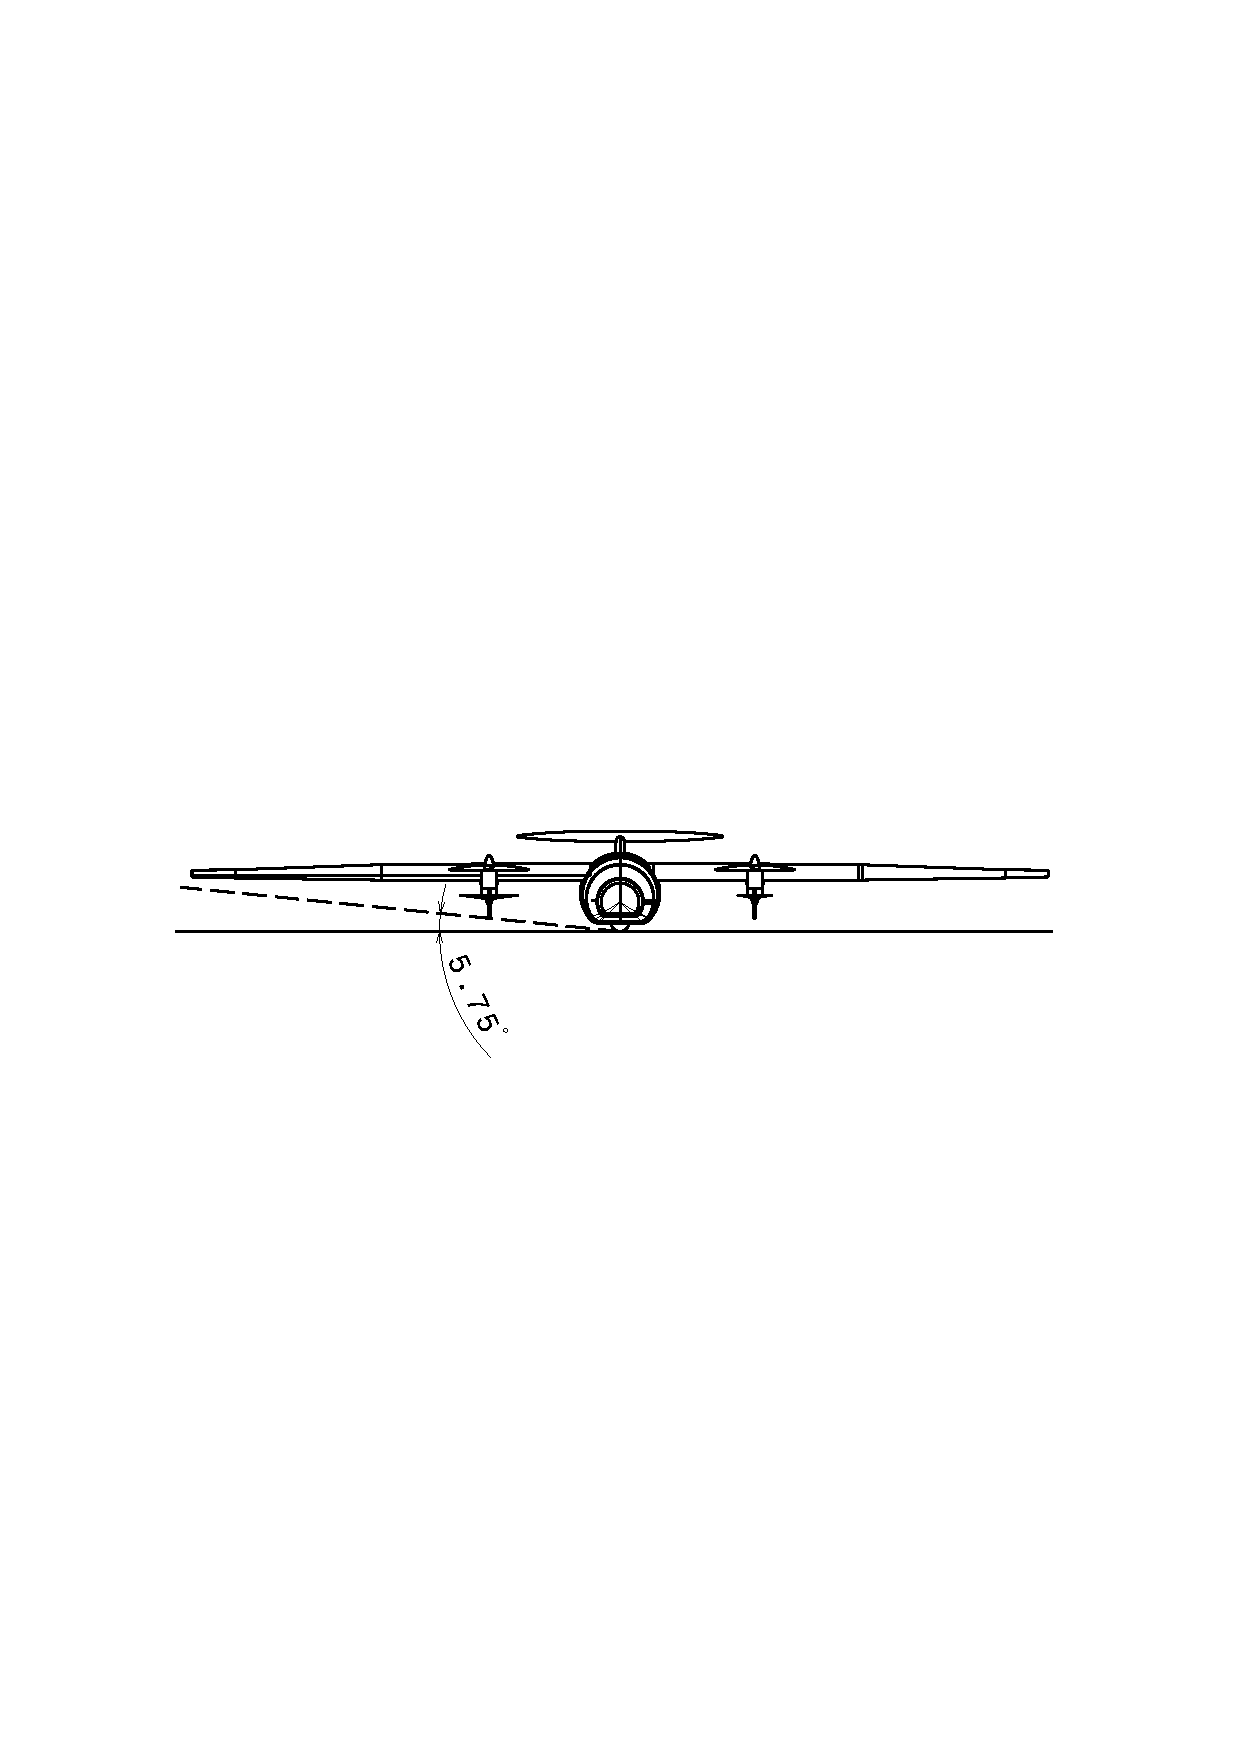
\includegraphics[width=0.75\textwidth]{Structures/Figures/ground_clearance}
    \caption{Ground Clearance}
    \label{fig:ground_clearance}
\end{figure}

% ---------------------------------------------------------------------------------------
\subsection{Integration}

In the previous sections all structural components that have been designed were presented separately, however, together they form a single subsystem of the UAV. \autoref{fig:complete_structure} shows the complete skeleton, which comprises the main wing, engine pylons, fuselage and the preliminary tail. As previously mentioned, the wing tips can be easily removed while the rest of the wing is rigidly connected to the fuselage frames. This configuration does not lead to the smallest possible transportation size, as can be seen also in \autoref{sec:oper_logi_conc_desc}, however, having uninterrupted parts where the loads are highest generally allows for a lighter design. Since the tail has not been designed in detail, also the connection to the fuselage is to be determined yet. It is expected though that the loads on the tail are introduced to the fuselage via the rearmost frame, which would need to be reinforced accordingly.



\begin{figure}[H]
    \centering
    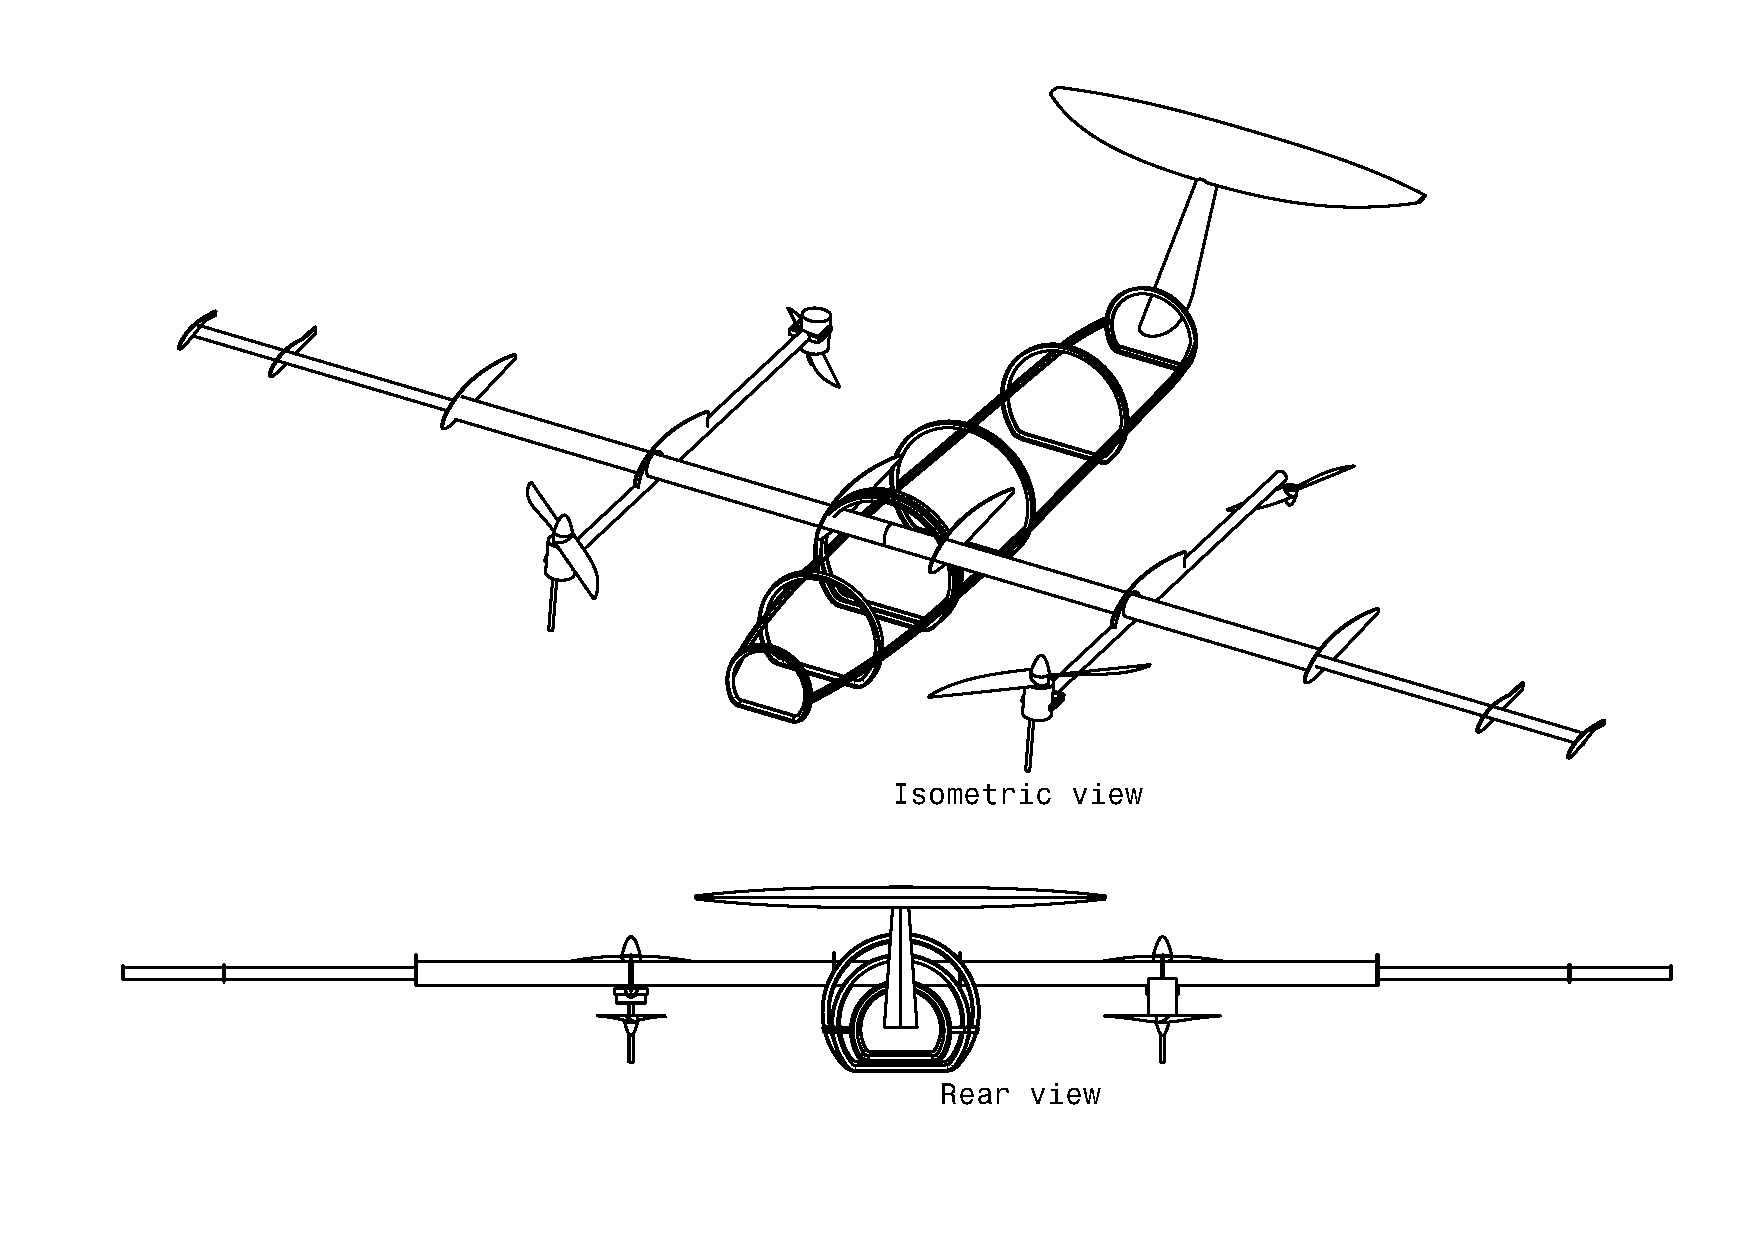
\includegraphics[width=0.75\textwidth]{Structures/Figures/Structure_iso}
    \caption{Internal structure of the UAV}
    \label{fig:complete_structure}
\end{figure}







% =======================================================================================
\section{Verification \& Validation}
\label{sec:veri_vali}
Verification of the tools used and validation of the resulting outcomes are of vital importance to the credibility of any analysis. In this section the verification and validation procedures for the structural analysis are described.

\paragraph{Loads}
The loads throughout the wing and fuselage were computed with Python scripts with the data retrieved from the master document. To verify these scripts they were subjected to unit testing methods. Simple loading cases comprising combinations of 1 N forces were analysed by the script and the resulting maximum and minimum shear force and bending moments as well as their locations were compared to calculations performed by hand. 

\paragraph{Stresses}
The stresses in the structural components of both the wing and fuselage were calculated using scripts written in Python. They used the loads calculated before, inputs from other subsystems and the geometry of the parts to evaluate the stresses in the structure.

The verification method for these scripts was similar to the one followed to verify the load calculations. Different loads and stringer locations were fed into the script to uncover a source of error. For a configuration in which some stringers where very close to the centroid of the cross-section erroneous boom areas resulted. This could be traced to a limitation of \autoref{eq:boom}, where the boom area will approach infinity as the distance of a given boom approaches the neutral axis. 

For the fuselage the results from the stress analysis were compared to the those from a calculation performed by hand. For this calculation the fuselage was simplified as a thin-walled tube with an equivalent diameter and was put under the same loads. This was not accurate enough to fully validate the results from the stress analysis. However, a more elaborate validation procedure was not possible within the given time constraints. Furthermore, the order of magnitude of the results was proven to be the same. In the future, an improved validation could be performed with a finite element method stress analysis on the CATIA model. 


\begin{comment}
verification:
unit, system testing for: load diagrams, bending and shear stress analyses
validation:
hand calculation known working model 
recommendation: validate on stress analysis Catia model
\end{comment}

% =======================================================================================

\begin{comment}

\section{Design Summary}
In this section the structural design resulting from the previously described process is presented. \autoref{fig:complete_structure} depicts the internal structure of the wing and fuselage. The main load carrying member in the wing is the carbon fibre tube which runs the entire span. Additionally, a series of spar webs guides loads onto this tube from the foam wing skin. At the intersection with the fuselage, two frames carry the torque and shear loads from the wing tube and transfer the loads to the stringers and skin. The fuselage skin is 0.5 mm thick and is made out of a glass fibre epoxy composite, as are the stringers and frames. In \autoref{fig:complete_structure} only two stringers are actually shown because the others could not be included into the CATIA model due to time constraints. The locations of the other stringers can still be found in \autoref{fig:stringers}.

\begin{figure}[H]
    \centering
    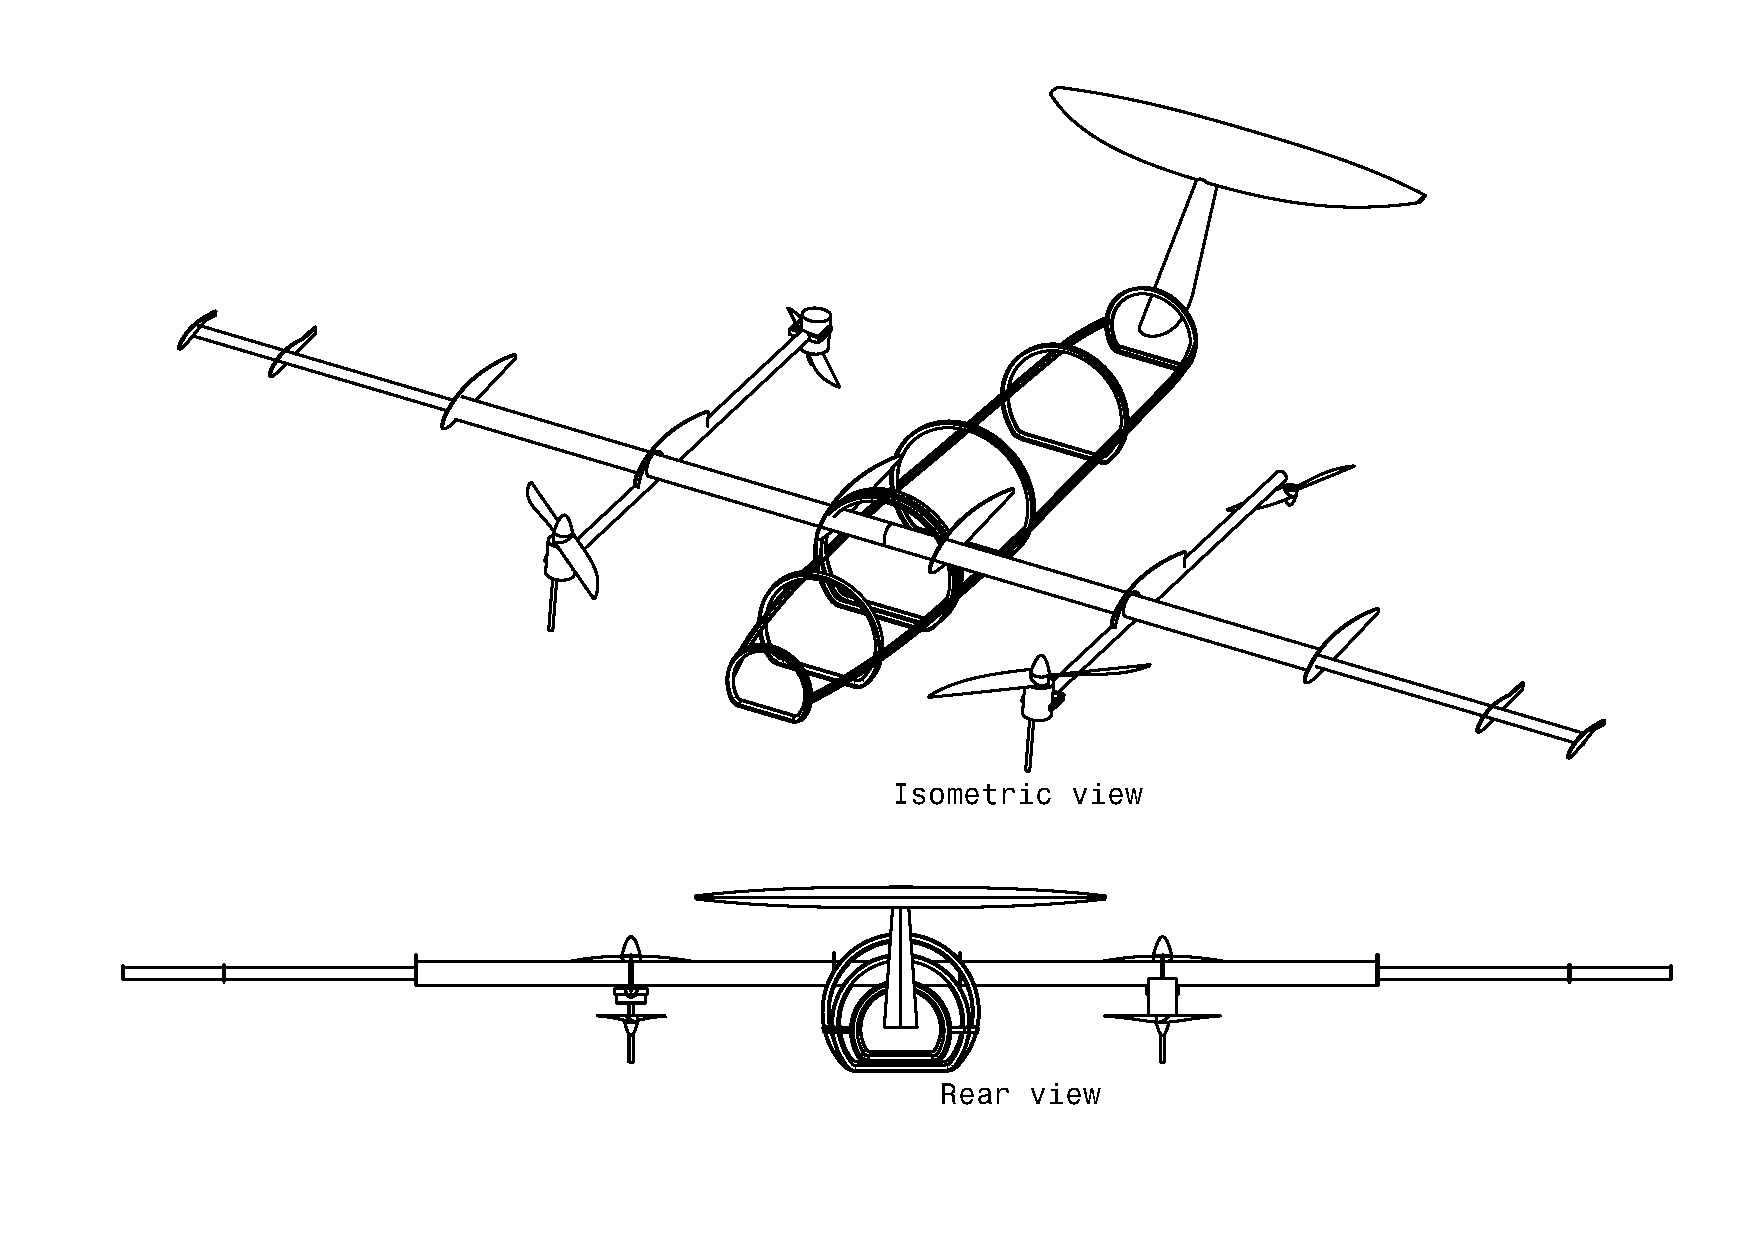
\includegraphics[width=0.75\textwidth]{Structures/Figures/Structure_iso}
    \caption{Internal structure of the UAV}
    \label{fig:complete_structure}
\end{figure}

\label{sec:resu_stru}
%%%%%%%%%%% THIS IS THE OLD PAYLOAD CHAPTER COMMENTED OUT FOR NOW %%%%%%%%%%

In this section, the fuselage and payload compartment design will be explained. First, the layout of the fuselage is presented. Based on this, a stress analysis is made. After that, different options for materials are compared. Finally, all design decisions, based on the previous analysis, are presented.


\section{Fuselage Layout}
\label{sec:fuse_layo}
Explain general layout of the fuselage, like where the torsion boxes, stringers etc will be located


\section{Stress Analysis}
\label{sec:stre_anal}




\section{Material Analysis}%Written by Steph
\label{sec:mate_anal}

In this section, an overview is given of different materials that could possibly be used to manufacture the UAV. Some relative qualities are presented for each material option. In \autoref{tab:mate_gene} all materials that contribute to the strength of the structure are given. In \autoref{tab:mate_clos} the possible materials for the payload bay closing system that do not contribute to the stress bearing capacities are compared. The cost is not discussed in these tables, since for the expected quantity of products, fibre reinforced composites can compete with steel\footnotemark.
\footnotetext{\url{http://msl1.mit.edu/MIB/3.57/LectNotes/gm_tech_composites.pdf}, Accessed 14-06-2017}



\begin{table}[h]
    \centering
    \caption{Overview of material options \cite{material}}
    \label{tab:mate_gene}
    \begin{tabularx}{\textwidth}{LCCC}
    \toprule
    \textbf{Skin} &  \textbf{Weight [g/$cm^3$] }  & \textbf{Thickness} & \textbf{Tensile strength}
    \\ \midrule
    Glass fibre composite    
    &  2.5 
    & 
    & 3.5 - 4.6 GPa\footnotemark
    \\ \hdashline
    Carbon fibre composite    & 1.8 & &
    \\ \hdashline
    Aluminium       & 2.7  & &
    \\ \hdashline
    Steel           & 7.9 & &
    \\ \hdashline
    Titanium        & 4.4 & &
    \\ \hdashline
    Kevlar          & 1.4 & &
    \\ \hdashline
    Wood            & 0.6 & &
    \\ \hdashline
    Plastic         & 1.2 & &
    \\ \hdashline
    Cloth           & & &
    \\ \bottomrule
    \end{tabularx}
\end{table}


\addtocounter{footnote}{2}
\stepcounter{footnote}\footnotetext{\url{https://www.researchgate.net/publication/265346634_Glass_fiber-reinforced_polymer_composites_-_A_review}, Accessed 14-06-2017} %flass fibre weight
\stepcounter{footnote}\footnotetext{\url{http://textilelearner.blogspot.nl/2012/09/glass-fiber-composites-properties-of.html}, Accessed 14-06-2017}%glass fibre strength


\section{Fuselage Design}




\paragraph{System Layout}
The closing system will consist of 
\end{comment}